\documentclass[12pt, titlepage]{article}
\usepackage{tikz}
\usepackage[skip=5pt plus1pt, indent=20pt]{parskip}
\usepackage{indentfirst}
\usepackage[utf8]{inputenc}
\usepackage[datesep=/,style=ddmmyyyy]{datetime2}
\usepackage{xcolor}
\usepackage[english]{babel}
\newcommand{\TODO}{\begin{center}\color{red}TODO\end{center}}
\usepackage{fancyhdr}
\pagestyle{fancy}

\title{Winning The "Graph Wars"}

\author{Artur Roos}

\date{\today}

\begin{document}
\maketitle
\tableofcontents

\section{Introduction}
\subsection{Rationale}
Not longer than two days ago I was challenged to a mathematical standoff by a 
good friend of mine, the weapons would be polynomial functions and their 
graphs. Winning this competition was a matter of honor, so I used all of my 
skill and wits to prepare. The fight would be held in \mbox{"Graphwar"}, a 
small competitive 1v1 game published on the 23rd of February 2022. 

The goal of the game is to design a function that can be plotted from one point
to another without intersecting any circles in shortest time. You are given 
60 seconds to input as many functions as you want, then the turn is passed onto
your opponent.
This is wrapped into a war-like setting where your function is a projectile, 
directed by your soldiers against your enemy's.

It is also usually played without assistance of any external programs like 
plotters or calculators, that's for good reason. Most importantly, game is
considered solved: for any initial state of the field there can be deduced a 
function to guarantee a "hit". 

\subsection{Aim}
My ultimate goal set out to be simply designing an algorithm, which when given
a list of all circle obstacles, their radii, and the edge points would express
the path to go from to another without colliding with any of the obstacles. 

The plane that the function is plotted on spans 40 units vertically and 
100 units horizontally. The units and the obstacles can only be placed at 
integer coordinates. 

You can sketch any function using the list of allowed 
operations:
\TODO


\section{Investigation}
The task consists of the small independents subtasks: finding the points and 
fitting the function. The found points are passed into the fitting algorithm,
so it in general it is a 2-step pipeline. Some alternative approaches use
more stages, as mentioned in the "Limitations \& Reflection" section. 

\subsection{Finding The Points}
This problem can be boiled down to pathfinding. However, usual pathfinding
techniques operate on discrete spaces like graphs and grids which our plane
is not, we need to convert it to one. Cells of the grid can be in two states:
occupied or empty. The occupied cells are the ones covered by an obstacle. 
Since obstacle circles only occur at integer coordinates and the smallest
radius of a circle is 1, we can safely assume that the smallest size of a grid
cell we might need is 1 respectively. After that we can apply the \textbf{Theta*}.
It is preferable to Dijkstra's, A* and others since it is designed to fit
any-angle pathfinding. It can find near-optimal paths with runtimes comparable
to A*. Even though our points are aligned on a grid,
the "projectile" is allowed to move in all directions, not just the cardinal ones. 
Only additional piece of information it requires is a line of sight function ($L$).
Let $I(A, B)$ be some function, equal to the amount of intersections of a 
line between points $A$ and $B$  with all the circles of a set $C$ containing 
$\langle x, y, r \rangle$. So $I_n(A, B)$ is the amount of intersections
of a line from $A$ to $B$ with some circle $C_n$. 
Using that we can define $I(A, B) = \sum_{n=1}^{|C|}I_n(A, B)$.

For simplicity let's assume the circle is at $\langle 0, 0 \rangle$ with
some radius $r$.
But first let's find the point $p_0 = (x_0, y_0)$ on the line closest to the circle.
We can use an alternative line equation $ax + by + c = 0$ for which we can for sure say that 
vector $\vec{v''} = (a, b)$ will be perpendicular to the line.

Coordiantes of $p_0$ should be proportional to the vector $\vec{v''}$. 
Now we may just normalize the vector to the length.

First we normalize by dividing the vector by it's length.
\begin{equation}
    \vec{v''}_{normalized}=\left(\frac{a}{\sqrt{a^2 + b^2}}, \frac{b}{\sqrt{a^2 + b^2}} \right)
\end{equation}
Then we scale the vector by the distance of the line to the origin.
\begin{equation}
    \vec{v'}=\vec{v''}_{normalized} * \frac{c}{\sqrt{a^2 + b^2}}
\end{equation}
By simplifying the denominators we get
\begin{equation}
    \vec{v}=\left(a * \frac{c}{a^2 + b^2}, b * \frac{c}{a^2 + b^2}\right)
\end{equation}

This vector is inverted, so by multiplying everything by $-1$ we get the actual 
coordinates of the point. Since the vector and the point lie in the same coordinate
system we can claim their equivalence, therefore
\begin{equation}
    p_0 = -\vec{v} = (-a * \frac{c}{a^2 + b^2}, -b * \frac{c}{a^2 + b^2}) = (x_0, y_0)
\end{equation}
So $p_0$ is the closest point to the circle.
Now, based on this we can calculate the amount of intersections: if $p_0$ is inside
the circle there are 2 intersections, it it lies on the radius there is 1 intersection
and there are none otherwise.
\begin{equation}
    \left\{\begin{array}{@{}l@{}}
       I_n(A, B) = 0, |\vec{v}| > C_{n_r}\\
       I_n(A, B) = 1, |\vec{v}| = C_{n_r}\\
       I_n(A, B) = 2, |\vec{v}| < C_{n_r}
    \end{array}\right.
\end{equation}
When evaluating the function $I_n$ for simplicity we just subtract the 
coordinates $(C_{n_x}, C_{n_y})$ from all the other coordinates. This shifts 
the entire plane so that the circle is at the origin, the precise usecase the
solution above covers.

Assuming the algorithm is not ill-formed and given correct input information
it should formulate a near-optimal path, some list $A$ of cardinality $n$, 
where each point is represted as  a pair of $x$ and $y$ coordinates 
$\langle x, y \rangle$. It is required that all points of $A$ satisfy 
$\forall a_i,a_{i+1} \in A : a_{i_x} < a_{{i+1}_x}$. If this is not true 
at some point the path turns back on itself. This game situation is unresolvable 
(more of that is mentioned in the "Limitations \& Reflection" section).

\subsection{Fitting The Function}

The fitting algorithm will operate on the list $A$, output by the 
pathfinding algorithm and assume the same ordering.

$A_n$ is guaranteed to be the rightmost point, which
will make the calculations a lot more intuitive.
We may also ignore all the $x$ values in ranges 
$(-\infty; a_{1_x})$ and $(a_{n_x}; \infty)$, since the function will not be 
evaluated there at any point.

There is an infinite number of ways to make a function that goes through a set of
points, the simplest one is construcing the Lagrange Interpolation Polynomial
which does fit this usecase perfectly. We may follow a specific example 
and try to generalise it later. 

For example $A = \{\langle 0, 1 \rangle, \langle 6, 9 \rangle, 
\langle 17, 4 \rangle, \langle 19, 22 \rangle\}$. All the coordinates are
purposfully picked to be in the first quadrant, since in this way they are
much easier to visualize.

First we may try to make a function $\phi_i(x)$ such that it equals to 0 at
every point, but $x_i$. For simplicity we may make it be equal to 1, this will
allow for better composability in the future. For example the process for 
the second point might look something like this.

First we use a helper function $\hat{\phi}_2(x)$ make it be zero at all the points, but $x_i$.
\begin{equation}
    \hat{\phi}_2(x) = (x - 0)(x - 17)(x - 19)
\end{equation}

Now the value at $x_2$ is non-zero, we can just devide it by $\hat{\phi}_2(x_2)$ 
so it is $1$ at $x_2$.

\begin{equation}
    \hat{\phi}_2(x_2) = \hat{\phi}_2(6) = (6 - 0)(6 - 17)(6 - 19)
\end{equation}
\begin{equation}
    \phi_2(x) = \frac{(x - 0)(x - 17)(x - 19)}{\hat{\phi}_2(x_2)}
\end{equation}

\begin{equation}
    \phi_2(x) = \frac{(x - 0)(x - 17)(x - 19)}{(6 - 0)(6 - 17)(6 - 19)}
\end{equation}

{
\centering
\begin{tabular}{c|c c c c}
    $x$ & $x_1$ & $x_2$ & $x_3$ & $x_4$ \\
    $\phi_2(x)$ & $0$ & $1$ & $0$ & $0$ \\
\end{tabular}\par
}

Formally, in this context $\phi_i$ is called a "Lagrange polynomial basis".
To make $\phi_i$ completely representative of the point at $x_i$ we need to 
scale it's vertical component by $y_i$. Let's define a new helper 
function $\psi_i(x)$.

\begin{equation}
    \psi_2(x) = y_2 \phi_2(x)
\end{equation}
\begin{equation}
    \psi_2(x) = \frac{(x - x_1)(x - x_3)(x - x_4)}{(x_2 - x_1)(x_2 - x_3)(x_2 - x_4)} * y_2
\end{equation}

Based on this we can express $\psi_i(x)$'s values for any $x_i$.

{
\centering
\begin{tabular}{c|c c c c}
    & $\psi_1(x) $ & $\psi_2(x)$ & $\psi_3(x)$ & $\psi_4(x)$ \\
    \hline
    $x_1$ & $y_1$ & $0$ & $0$ & $0$ \\
    $x_2$ & $0$ & $y_2$ & $0$ & $0$ \\
    $x_3$ & $0$ & $0$ & $y_3$ & $0$ \\
    $x_4$ & $0$ & $0$ & $0$ & $y_4$ \\
\end{tabular}\par
}

Looking at the table of all the values of $\psi_i$ we can deducde that their linear
combination will satisfy our condition of $\psi_i(x_i) = y_i$ and 
$\psi_i(x_j) = 0, j \neq i$, yielding an $|A|$th order polynomial. 
So for the example set $A$ the fit function is 
$f(x) = \psi_1(x) + \psi_2(x) + \psi_3(x) + \psi_4(x)$.

If we generalise this function to any set $A$ it would look
like the following.

\begin{equation}
    f(x) = \sum_{i=1}^{|A|}\psi_i(x)
\end{equation}

We can also expand our helper functions $\phi$ and $\psi$, so we get it to our 
final form.
$$\psi_i(x) = y_i \phi_i(x)$$
\begin{equation}
    \phi_i = \prod_{j=1, j \neq i}^{|A|}\frac{x - x_j}{x_i - x_j}
\end{equation}

The final form is the following, a proper Lagrange Interpolation Polynomial,
a member of $P_n$. The 
\begin{equation}
f(x) = \sum_{i=1}^{|A|} \left(y_i * \prod_{j=1, j \neq i}^{|A|} \frac{x - x_j}{x_i - x_j}\right)
\end{equation}

This is the final form of the function $f$, that given a set of points 
fits a function through them. When applying it in practise one should 
not forget to account for the previously applied transformations, such as 
the offset of the soldier's origin. It's (na\"ive) computational complexity
is $O(n^2)$, which is subpar, possible improvements are mentioned in the 
"Limitations \& Reflection" section.

\section{Limitations \& Reflection}
I used a geometric approach to finding intersections of lines with circles.
The algebraic solution has a higher computational error due to imprecisions 
of floating-point arithmetic. This doesn't impact the current usecase,
however can be important when dealing with more fine point placement.

The origin of each soldiers' shot is unique. The $x$ 
coordinate is $0$, but the $y$ is same as that of the soldier. The investigation
conciously ignores this restriction since it would make the solution overwhelming
and difficult to read. Accounting for that requires subtracting the soldier's 
position from the each of the path points.

The described method of fitting covers a lot of scenarios, but it doesn't yield 
correct results
when the next intended path point $a_{i + 1}$ on the path which goes after 
some $a_i$. In this case the pathfinding algorithm requires a path to turn back,
which is impossible to do. This issue is most visible when reindexing: the order
of points will be changed. Beyond that, this arises only in situations when the 
$f(x)$ \textbf{can't be a well-defined function}, since that requires it to have to
two different values at same $x$. Luckily, those scenarios never occured in a 
real game. Perhaps the game accounts for that and intentionally avoids it.

My method produces good results on the given dataset of densely packed points,
however, the more spread apart the points are the greater the algorithm
overshoots in spaces between two points. That can be a problem since it may 
actually accidentally go through one of the spheres. This effect can be
mitigated by sampling more intermediate points, which in turn increases 
computational complexity. Since the game field is  limited to span 100 units
horizontally and 40 units vertically this is not a big problem. One of the
alternative solutions would be using splines to form B\'{e}zier Curves, 
Hermite Curves, Catmul-Rom or even B-Splines, but those are \textbf{barely touched 
on in the book} if at all. Using splines would be optimal, beyond that
a spline of degree $\infty$ for a set of points \textit{is} the Lagrange
Interpolation. I would really love for them to be included in the cirruculum.

All the solutions later developed by other people interested in the game employ
similar approaches with some optimisations on the algorithm side. Some also
make use of CV (Computer Vision) to automatically dispatch the data to the
calculator which later forms a polynomial. Several applications use
an additional step of the pipeline to optimise the resulting polynomial
by approximating it further using other techniques.

In some edge-case scenarios errors in floating point arithmetic might 
cause an unintentional collision. Since built paths might be touching 
the radius of the circle (due to the nature of the algorithm) it might be
useful to artifically increase the radius through some function $h(r) = r + t$,
to ensure that the path is built at least $t$ units away from the cirles.

\section{Conclusion}
In conclusion I can for sure regard this research as successful. All the
described techniques were applied and achieved great results. I won the
standoff and got to explain my methodology to the defeated opponent, which
was delightful. Beyond that, several possible improvements were already 
mentioned above. I would be interested in redoing that research in some time
to see how my understanding of the topic has changed with the knowledge I will
develop.

\begin{center}
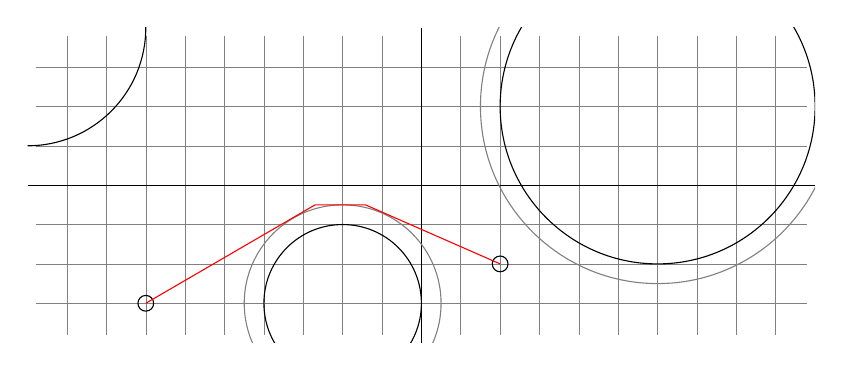
\begin{tikzpicture}[scale=0.1]
    \clip (-50,-20) rectangle (50,20);
    \draw[step=5,gray,very thin] (-49,-19) grid (49,19);
    \draw (-50,0) -- (50,0);
    \draw (0,-20) -- (0,20);
    
    \draw (-35,-15) circle [radius=1cm]; %me
    \draw (10,-10) circle [radius=1cm]; %them
    
    \draw (-10,-15) circle [radius=10cm];
    \draw[gray] (-10,-15) circle [radius=12.5cm];
    \draw (-50,20) circle [radius=15cm];
    \draw[gray] (-50,20) circle [radius=172.5cm];
    \draw (30,10) circle [radius=20cm];
    \draw[gray] (30,10) circle [radius=22.5cm];

    \draw[red] plot coordinates {(-35,-15) (-13.5,-2.5) (-7.1,-2.5) (10,-10)};
    \draw[color=blue,domain=-20:0] plot[mark=x,smooth] file {plots/conclusion-function.table};
\end{tikzpicture}
\end{center}
A representation of a game field with function $f$ generated using my
algorithm. The radii provded to the algorithm were increased by 2.5,
they are drawn in gray. The path generated by Theta* is drawn in red.
The path of the generated function is in blue. In this specific case
the simplified polynomial is like this (the entire process of expansion
is ommited for the sake of brevity, it  would take an unreasonable amount 
of time to compute manually and an unreasonable amount of paper to print).

% smaller dots
\newcommand\smalldots{\makebox[0.75em][c]{.\hfil.\hfil.}}

$$f(x) = 4.833\smalldots \times 10^{-5} x^3- 1.181\smalldots{} \times 10^{-2} x^2 - (0.389\smalldots{}) x - 4.335\smalldots \textcolor{gray}{+ 15}$$

The last term is the offset of the soldier from origin and is not part of the
Lagrange Interpolation, however it plays an important role in the game and 
is not to be forgotten about.

\TODO

\section{Bibliography}
\appendix
\TODO

\end{document}
